\documentclass{beamer}
\usepackage{amsmath}
\usepackage{subfig}
\usepackage{tikz}
\captionsetup[subfigure]{labelformat=empty}
\usepackage{graphicx}
\usetikzlibrary{positioning}
\usepackage{cmbright}
\usepackage[table,x11names]{xcolor}
\usepackage{multirow}
\usepackage{xhfill}
\mode<presentation>
{
  \usetheme{Amsterdam}
  \setbeamercovered{transparent}
  \beamertemplatenavigationsymbolsempty
}
\renewcommand{\textquotedbl}{\texttt{"}}
\newcommand{\ditto}[1][.4pt]{\xrfill{#1}~\textquotedbl~\xrfill{#1}}

\setbeamertemplate{footline}
{
  \leavevmode%
  \hbox{%
  \begin{beamercolorbox}[wd=.333333\paperwidth,ht=2.25ex,dp=1ex,center]{author in head/foot}%
    \usebeamerfont{author in head/foot}\insertshortauthor % Get rid of short institute next to name
  \end{beamercolorbox}%
  \begin{beamercolorbox}[wd=.333333\paperwidth,ht=2.25ex,dp=1ex,center]{title in head/foot}%
    \usebeamerfont{title in head/foot}\insertshorttitle
  \end{beamercolorbox}%
  \begin{beamercolorbox}[wd=.333333\paperwidth,ht=2.25ex,dp=1ex,right]{date in head/foot}%
    \usebeamerfont{date in head/foot}\insertshortdate{}\hspace*{2em}
    \insertframenumber{} / \inserttotalframenumber\hspace*{2ex} 
  \end{beamercolorbox}}%
\vskip0pt%
} \makeatother \setbeamercovered{dynamic}
\title[Object Retrieval]
{Feature-Feature Matching For Object Retrieval in Point Clouds}

\author[Michal Staniaszek]{\large{Michal Staniaszek} \\
  \scriptsize{Supervisor: John Folkesson}}
\institute[KTH]{Royal Institute of Technology}
\setcounter{tocdepth}{1}

\date{\today}

\AtBeginSection[]
{
 \begin{frame}<beamer>
 \frametitle{Outline}
 \tableofcontents[currentsection]
 \end{frame}
}

\begin{document}
\begin{frame}
  \titlepage
\end{frame}

\begin{frame}{Outline}
  \tableofcontents
\end{frame}

\section{Introduction}
\begin{frame}{What is object retrieval?}
  \begin{center}
    \textbf{Finding object locations in point clouds}
  \end{center}
  \vspace{0.25cm}
  Can use knowledge about objects to
  \begin{itemize}
  \item Determine the type of room one is in
  \item Find object in order to perform a task with it
  \item Predict or track object position over time
  \end{itemize}
  Many of these useful in household/office applications
  
  \vspace{0.25cm}
  Two main approaches
  \begin{itemize}
  \item Feature matching: match low level representations of objects
  \item Model matching: match entire object or high level representation
  \end{itemize}
\end{frame}
\begin{frame}{This Project}
  Focus on feature matching, implement system for object retrieval. Working with
  3D dataset.
  
  \vspace{0.5cm}
  Questions that the project aims to investigate:
  \begin{itemize}
  \item Can naive representations be effective?
  \item Which representations are best?
  \end{itemize}
\end{frame}
\begin{frame}{System Structure}
  \centering
  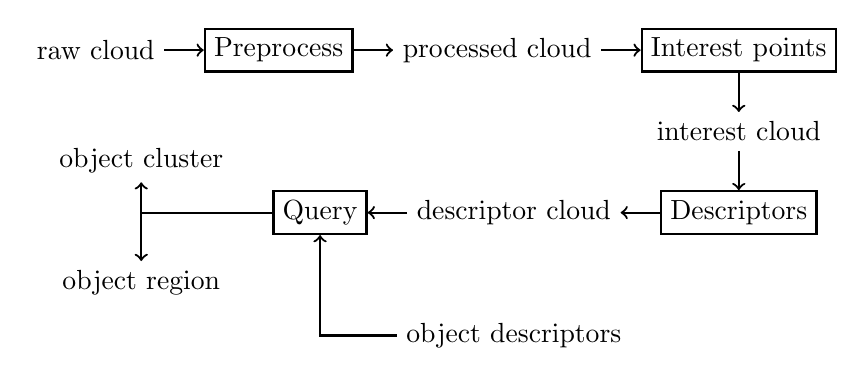
\begin{tikzpicture}
    \node[] (raw) {raw cloud};

    \node[draw,rectangle,thick,right=0.5cm of raw] (pre) {Preprocess};
    \node[right=0.5cm of pre] (proc) {processed cloud};
    \node[draw,rectangle,thick,right=0.5cm of proc] (interest) {Interest points};
    \node[below=0.5cm of interest] (intc) {interest cloud};
    \node[draw,rectangle,thick,below=0.5cm of intc] (desc) {Descriptors};
    \node[left=0.5cm of desc] (desccl) {descriptor cloud};
    \node[draw,rectangle,thick,left=0.5cm of desccl] (query) {Query};
    \node[above left=0.1cm and 0.5cm of query] (cluster) {object cluster};
    \node[below=1cm of cluster] (region) {object region};

    \node[below=1cm of desccl] (objdesc) {object descriptors};
    
    % arrows
    \draw[->,thick] (raw) -- (pre);
    \draw[->,thick] (pre) -- (proc);
    \draw[->,thick] (proc) -- (interest);
    \draw[->,thick] (interest) -- (intc);
    \draw[->,thick] (intc) -- (desc);
    \draw[->,thick] (desc) -- (desccl);
    \draw[->,thick] (desccl) -- (query);
    \draw[->,thick] (query) -| (cluster);
    \draw[->,thick] (query) -| (region);
    \draw[->,thick] (objdesc) -| (query);

  \end{tikzpicture}
\end{frame}
\section{Preprocessing}
\begin{frame}{Data}
  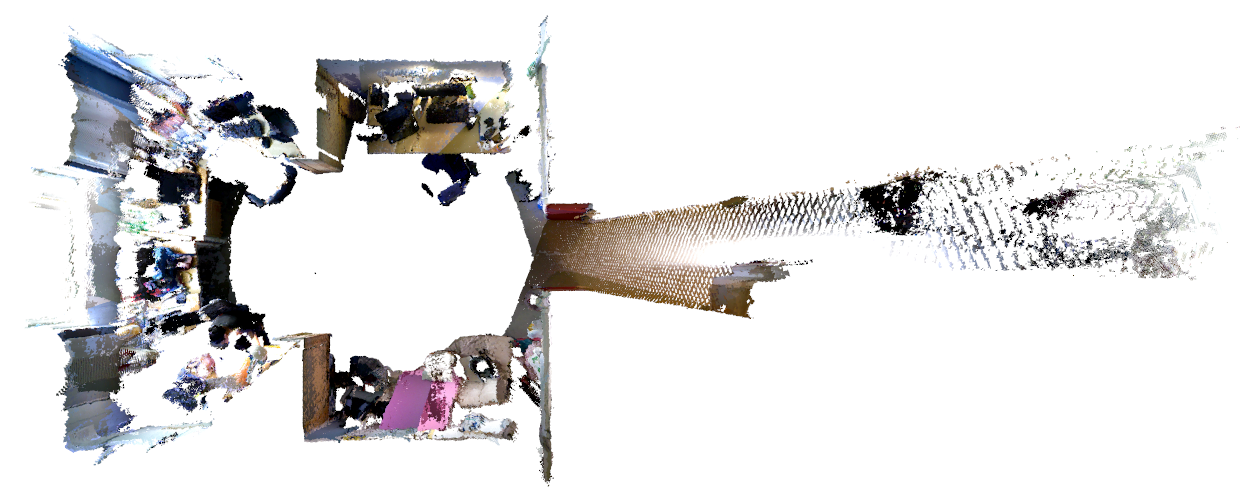
\includegraphics[width=0.49\textwidth]{images/orig_top}
  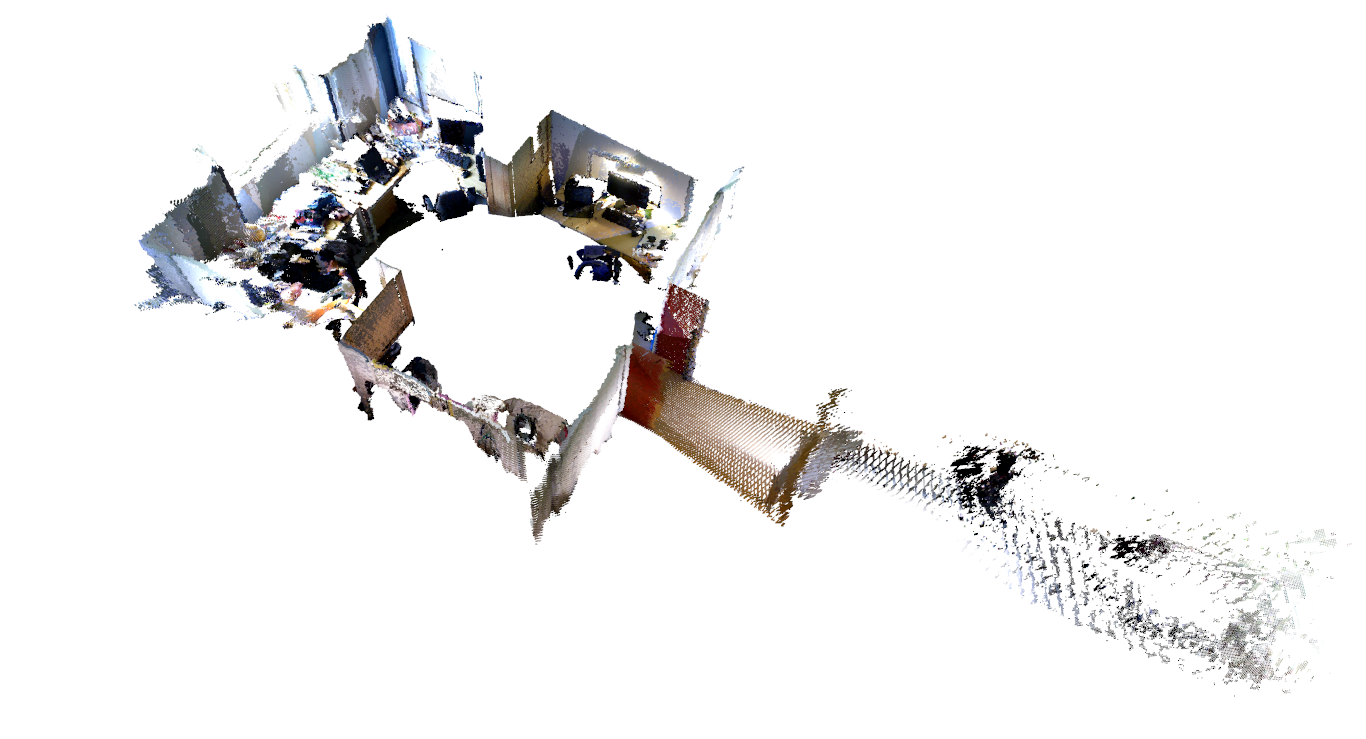
\includegraphics[width=0.49\textwidth]{images/orig_diag_left}
  
  Data set consists of:
  \begin{itemize}
  \item Full scans of a room over 1 month
  \item Scans constructed from intermediate frames
  \item Labels for some persistent objects in the rooms
  \end{itemize}
  Can exploit the fact that dataset has known structure, but also want to
  generalise.
\end{frame}
\begin{frame}{Downsampling, transformation and trimming}
  \begin{center}
    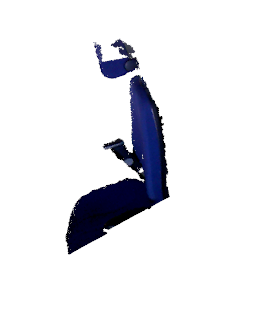
\includegraphics[width=0.2\textwidth]{images/annotations/slices/chair_front}
    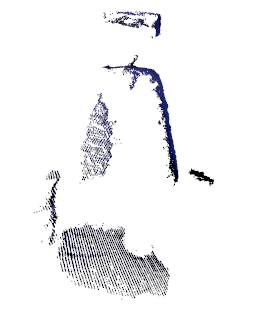
\includegraphics[width=0.2\textwidth]{images/annotations/slices/chair_side}
    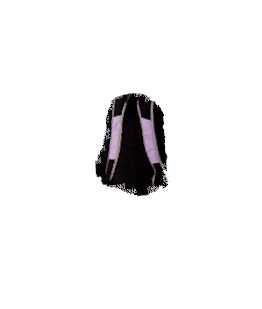
\includegraphics[width=0.2\textwidth]{images/annotations/slices/backpack_front}
    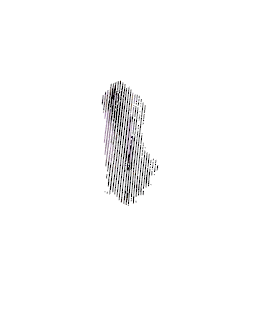
\includegraphics[width=0.2\textwidth]{images/annotations/slices/backpack_side}
  \end{center}
  Clouds have approx. 4mil points.
  \begin{itemize}
  \item Need to reduce this for more efficient processing
  \item Can help reduce noise and slicing effects
  \end{itemize}
\end{frame}
\begin{frame}
  \begin{center}
    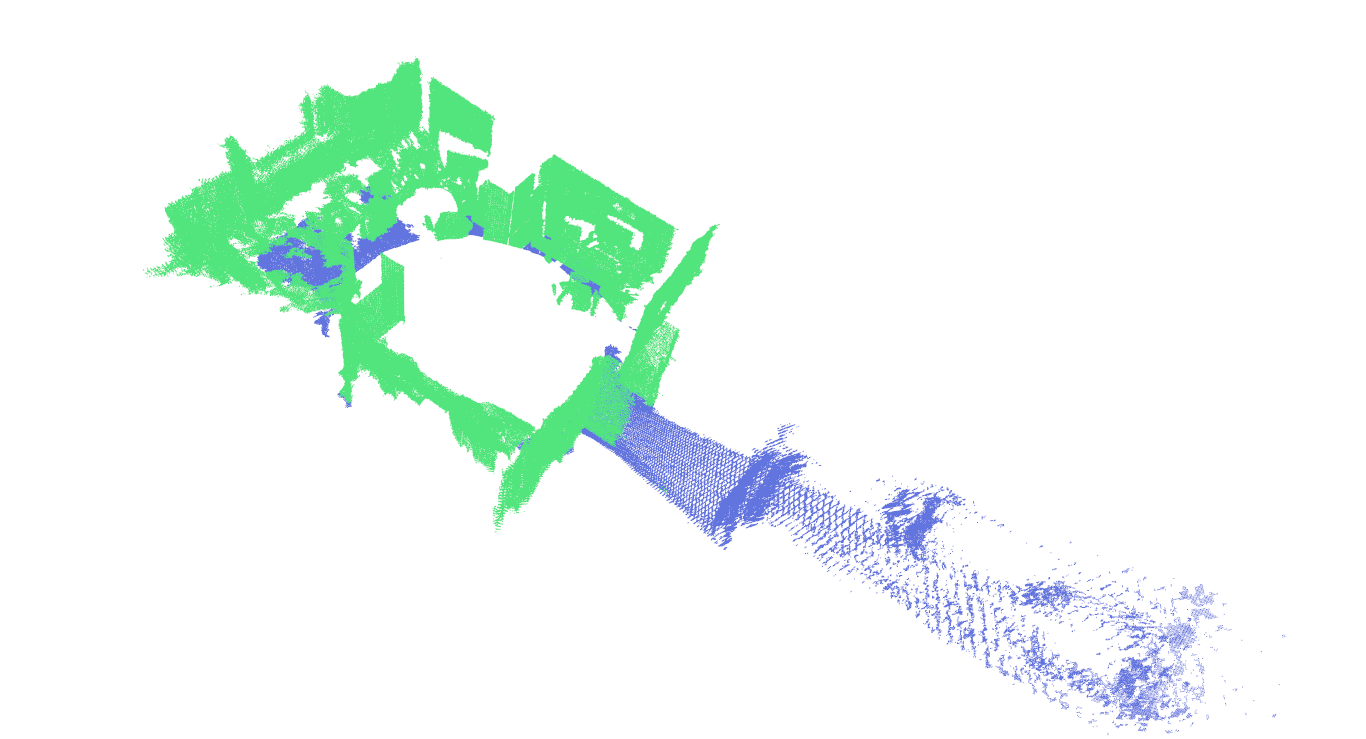
\includegraphics[width=0.8\textwidth]{images/trimmed_diag_left}\\
    
\includegraphics[width=0.8\textwidth]{images/trimmed_side}
  \end{center}
\end{frame}
\begin{frame}{Plane Extraction}
  Apply RANSAC to trimmed clouds multiple times
  \begin{itemize}
  \item Remove walls, desks and other flat surfaces
  \item These are not likely to be part of objects
  \end{itemize}
  Different plane models; with or without normals
  \begin{itemize}
  \item With normals is better, but requires adjustment of the normal radius
  \end{itemize}
\end{frame}
\begin{frame}
  \begin{figure}
    \centering
    \subfloat[Simple plane]{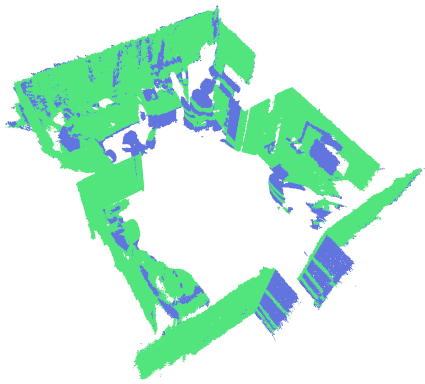
\includegraphics[width=0.49\textwidth]{images/plane_nonorm}}
    \subfloat[Plane with normal]{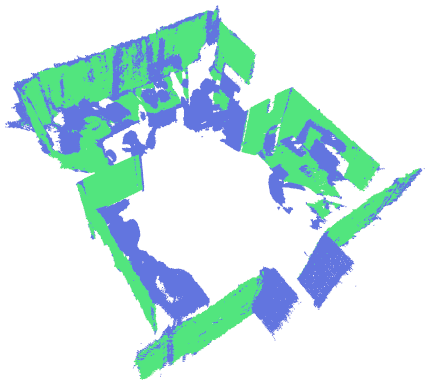
\includegraphics[width=0.49\textwidth]{images/plane_withnorm}}
  \end{figure}
\end{frame}
\begin{frame}
  \vspace{-0.5cm}
  \begin{figure}
    \centering
    \subfloat[0.02]{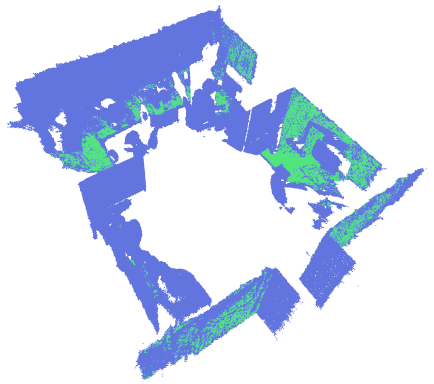
\includegraphics[width=0.35\textwidth]{images/plane_normal_0,02}}
    \subfloat[0.04]{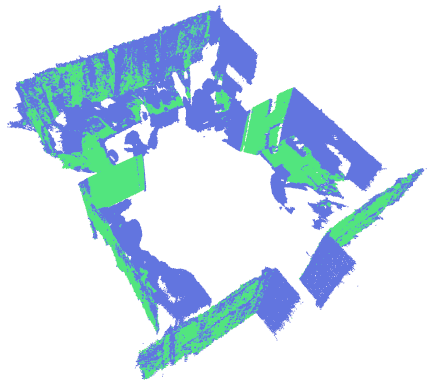
\includegraphics[width=0.35\textwidth]{images/plane_normal_0,04}}\\
    \subfloat[0.06]{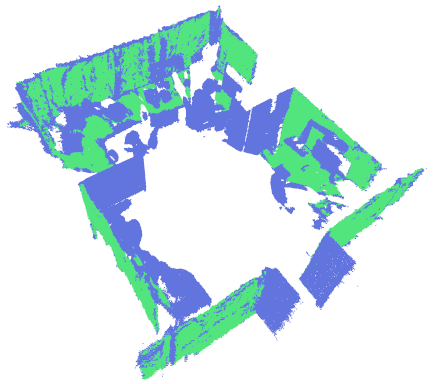
\includegraphics[width=0.35\textwidth]{images/plane_normal_0,06}}
    \subfloat[0.08]{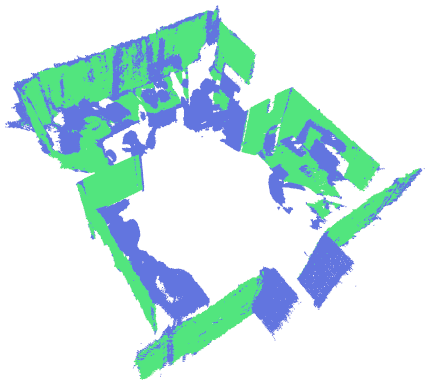
\includegraphics[width=0.35\textwidth]{images/plane_withnorm}}
  \end{figure}
\end{frame}
\begin{frame}
  % 20140903/patrol_run_14/room_1
  \begin{center}
    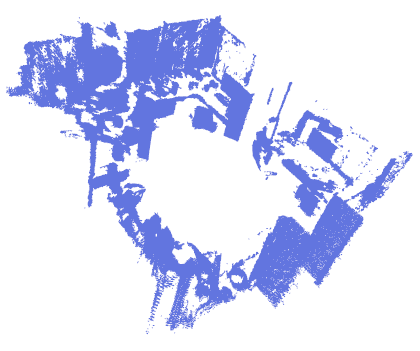
\includegraphics[width=0.8\textwidth]{images/nonplanes}
  \end{center}
\end{frame}

\section{Interest Points}
\begin{frame}
  \textbf{Q:} Where does one compute features? \textbf{A:} ``Interesting'' points

  Interesting points usually defined by:
  \begin{itemize}
  \item Minima/maxima of certain properties
  \item e.g. curvature, intensity, point covariances
  \end{itemize}
  
  Increasing complexity:
  \begin{description}
  \item[Uniform:] Voxel grid
  \item[ISS:] Scatter matrix
  \item[SUSAN:] Size of similar regions
  \item[SIFT:] Difference of Gaussians over scales
  \end{description}
\end{frame}
\begin{frame}
  \vspace{-0.5cm}
  \begin{figure}
    \centering
    \subfloat[Uniform]{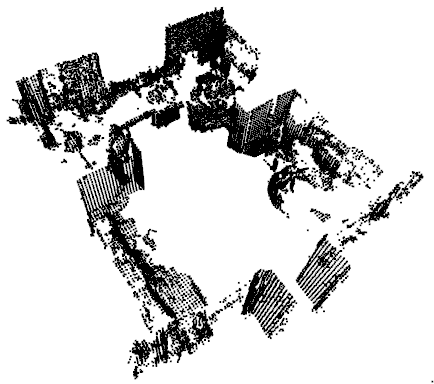
\includegraphics[width=0.35\textwidth]{images/uniform_points}}
    \subfloat[ISS]{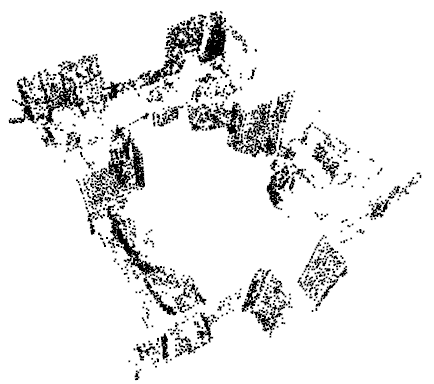
\includegraphics[width=0.35\textwidth]{images/iss_points}}\\
    \subfloat[SUSAN]{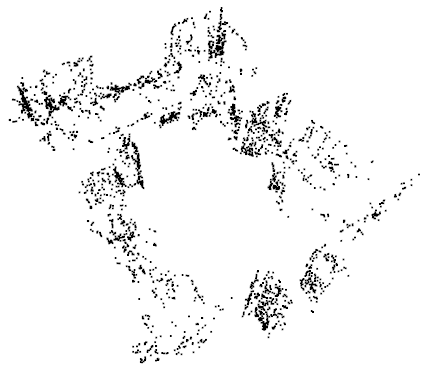
\includegraphics[width=0.35\textwidth]{images/susan_points}}
    \subfloat[SIFT]{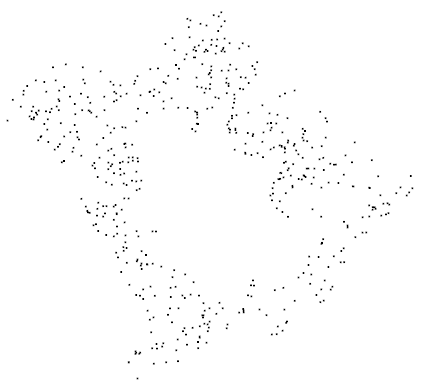
\includegraphics[width=0.35\textwidth]{images/sift_points}}
  \end{figure}
\end{frame}
\section{Descriptors}
\begin{frame}{What is a descriptor?}
  Used to represent regions in image or point cloud
  \begin{itemize}
  \item Compresses information about the region
  \item Simplifies comparison between regions
  \end{itemize}
  Desirable qualities:
  \begin{itemize}
  \item Similar regions produce similar descriptors
  \item Noise tolerance
  \item Unique reference frame (scale/rotation invariance in 2D)
  \end{itemize}
  Create compact representations of query and target clouds and compare them.
\end{frame}
\begin{frame}{SHOT descriptors}

  \begin{columns}
    \begin{column}{0.5\textwidth}
      Computation:
      \begin{itemize}
      \item Select central point $p$
      \item Find cosine of angle between normal $p$ and neighbours within radius
        $R$
      \item Add to local histogram bins
      \item Combine local histograms
      \end{itemize}
      SHOTCOLOR extends the above by adding the $L_1$ norm of the colour values
      to the shape description histogram
    \end{column}
    \begin{column}{0.5\textwidth}
      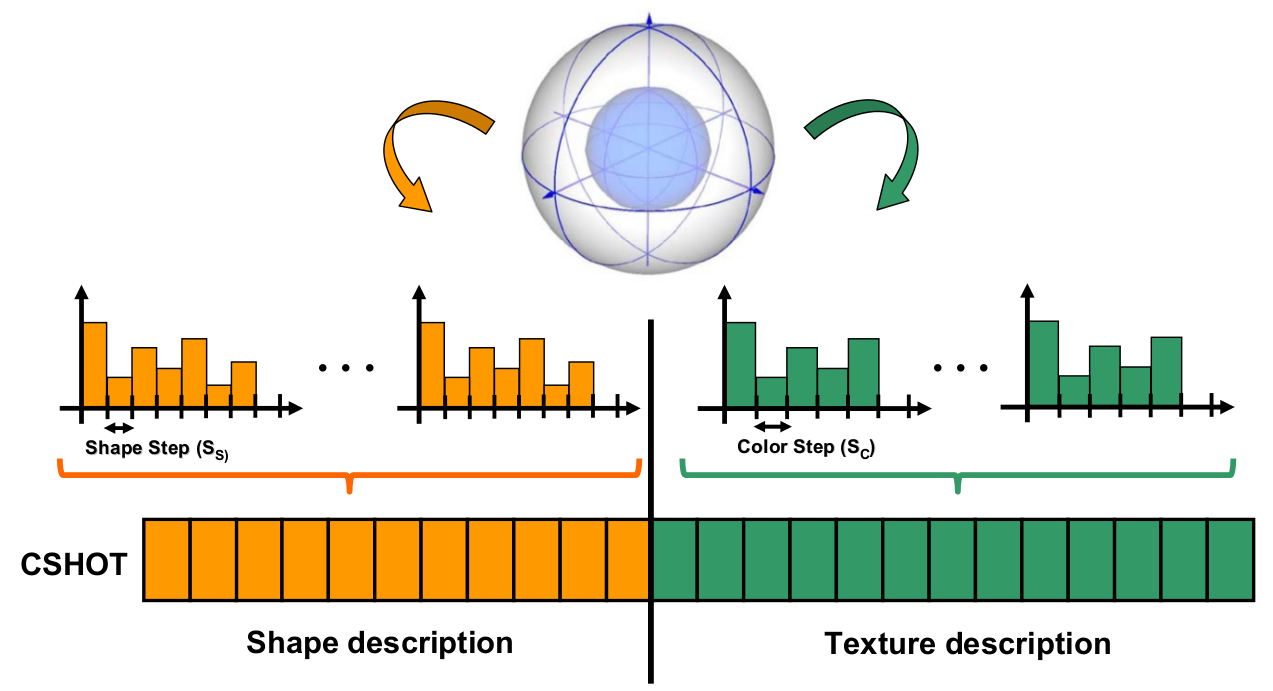
\includegraphics[width=\textwidth]{images/shotcolor}
    \end{column}
  \end{columns}
\end{frame}
\begin{frame}{PFH descriptors}
    \begin{columns}
    \begin{column}{0.5\textwidth}
      Computation:
      \begin{itemize}
      \item Look at all pairs of points in radius $R$
      \item Define coordinate frame using normal
      \item Compute 4 features based on angles and distances between the two points
      \item Increment histogram based on index from feature combination
      \end{itemize}
    \end{column}
    \begin{column}{0.5\textwidth}
      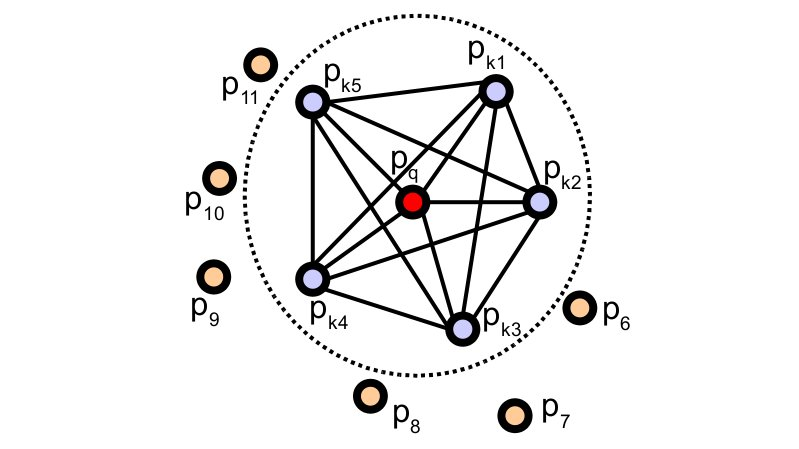
\includegraphics[width=\textwidth]{images/pfh}
    \end{column}
  \end{columns}
\end{frame}
\begin{frame}{PFH extensions}
    \begin{columns}
    \begin{column}{0.5\textwidth}
      FPFH:
      \begin{itemize}
      \item Look at point pairs within radius of each point instead of all pairs
      \item Concatenate separate feature histograms instead of indexing (reduce redundancy)
      \end{itemize}
      PFHRGB:
      \begin{itemize}
      \item Adds 3 features for ratio of colour values between points
      \end{itemize}
    \end{column}
    \begin{column}{0.5\textwidth}
      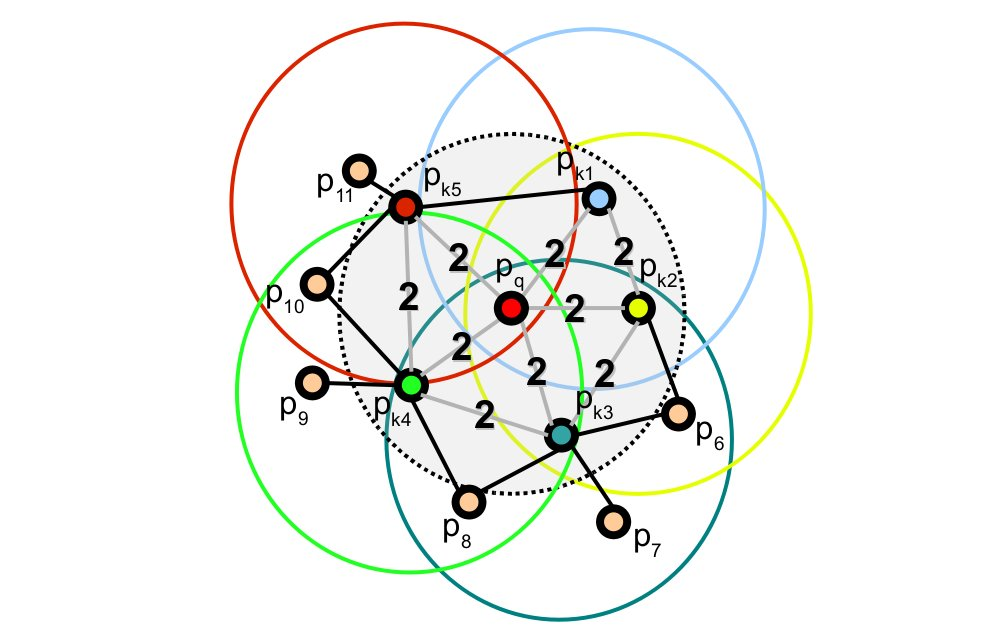
\includegraphics[width=\textwidth]{images/fpfh}
    \end{column}
  \end{columns}
\end{frame}
\section{Object Query}
\begin{frame}{Query objects}
  Query objects are:
  \begin{itemize}
  \item Instances of objects taken from annotation clouds
  \item Assumed to contain only points on the object
  \end{itemize}
  Could use individual frames for input, but
  \begin{itemize}
  \item Would require segmentation to extract object
  \item Would likely be less accurate, since frame can contain multiple objects and also non-objects
  \end{itemize}
\end{frame}
\begin{frame}{Matching}
  Find closest $K$ descriptors to each point in the query cloud.
  \begin{itemize}
  \item Distances found using simplified $L_2$ norm
  \item Comparing query to target means all query points have a nearest neighbour in target.
  \item No point finding neighbours for each target point --- for most target
    points, point in query likely to be far away
  \end{itemize}
  Output of this step is a list of nearest neighbours for each point
\end{frame}
\begin{frame}{Voting}
  Construct 3D grid and populate cells with values
  \begin{itemize}
  \item Each descriptor has an associated point in 3D space
  \item Increment cell containing point for each descriptor in nearest neighbour
    list
  \item Each cell represented by its centre point
  \end{itemize}
\end{frame}
\begin{frame}
  \begin{center}
    %20140908/patrol_run_38/room_2
    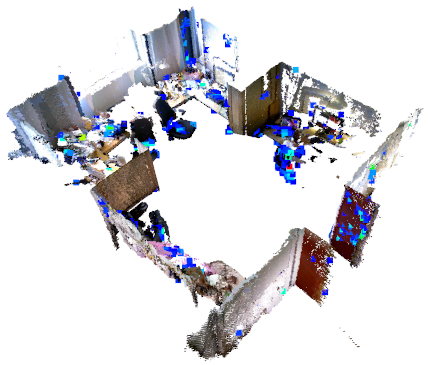
\includegraphics[width=0.8\textwidth]{images/votes_pfhrgb}
  \end{center}
\end{frame}
\begin{frame}
  \begin{center}
    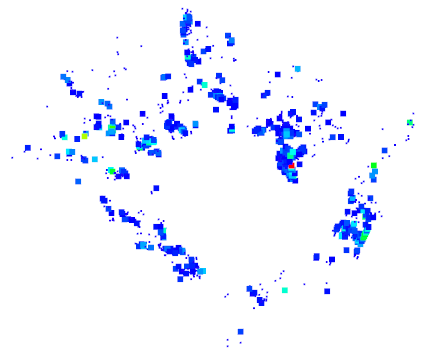
\includegraphics[width=0.8\textwidth]{images/votesonly_pfhrgb}
  \end{center}
\end{frame}
\begin{frame}{Clustering}
  Use cells with top $N$ number of votes to cluster
  \begin{itemize}
  \item Assume that the top votes are likely to be on matching objects
  \item Regions with many points in the top votes are likely to be on the object
  \item Use Euclidean clustering on the top points
  \item Clusters sorted based on summed score of points they contain
  \item Centroid of cluster used to extract region from target cloud
  \end{itemize}
\end{frame}
\begin{frame}
    \begin{center}
    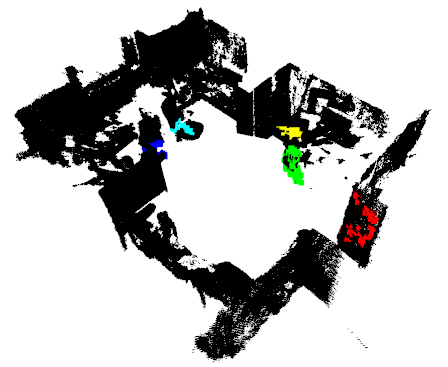
\includegraphics[width=0.8\textwidth]{images/clusters_pfhrgb}
  \end{center}
\end{frame}
\begin{frame}
  \begin{figure}
    \centering
    \centerline{
      \subfloat[Original]{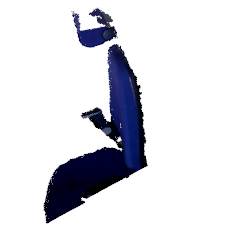
\includegraphics[width=0.2\textwidth]{images/annotations/original/chair1_front_ut.png}}
      \subfloat[526 votes]{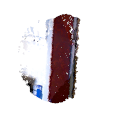
\includegraphics[width=0.2\textwidth]{images/pfhrgb_region_0}}
      \subfloat[458 votes]{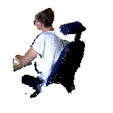
\includegraphics[width=0.2\textwidth]{images/pfhrgb_region_1}}}\\
    \centerline{
      \subfloat[295 votes]{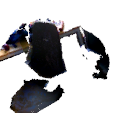
\includegraphics[width=0.2\textwidth]{images/pfhrgb_region_2}}
      \subfloat[118 votes]{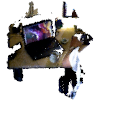
\includegraphics[width=0.2\textwidth]{images/pfhrgb_region_3}}
      \subfloat[116 votes]{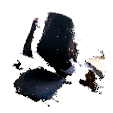
\includegraphics[width=0.2\textwidth]{images/pfhrgb_region_4}}}
  \end{figure}
\end{frame}
\section{Experimental Results}
\begin{frame}{Experimental Setup}
  \begin{itemize}
  \item Run preprocessing on all clouds using several settings 
  \item Compute descriptor and interest point combinations on these settings
  \item Run query on 7 objects using settings of the above, and vary query
    parameter settings
  \end{itemize}
\end{frame}
\begin{frame}{Cloud size reduction from preprocessing}
  \begin{table}
    \centering
    \small
    \centerline{
      \begin{tabular}{r|ccccc}
        Setting & Downsample & Trim & Trim Orig & Plane & Plane Orig \\\hline
        DEF & 0.23$\pm$0.01 & 0.79$\pm$0.01 & 0.18$\pm$0.00 & 0.50$\pm$0.06 & 0.09$\pm$0.01 \\ 
        DS15 & 0.11$\pm$0.00 & 0.76$\pm$0.02 & 0.08$\pm$0.00 & 0.67$\pm$0.12 & 0.06$\pm$0.01 \\
        DS2 & 0.06$\pm$0.00 & 0.74$\pm$0.02 & 0.05$\pm$0.00 & 0.89$\pm$0.07 & 0.04$\pm$0.00 \\
      \end{tabular}
    }
  \end{table}
\end{frame}  
\begin{frame}{Time taken for preprocessing}
  \begin{table}
    \small
    \centering
    \centerline{
      \begin{tabular}{c|llll}
        Setting & Normals        & Planes            & PerPlane        & Total \\\hline       
        DEF     & 16.33$\pm$1.11 & 116.12$\pm$13.63  & 15.10$\pm$1.43  & 133.32$\pm$14.13 \\  
        DT      & 12.29$\pm$1.30 & 114.30$\pm$18.81  & 13.69$\pm$1.65  & 127.35$\pm$19.44 \\  
        RI500   & 13.20$\pm$1.23 & 262.81$\pm$60.10  & 34.19$\pm$9.00  & 278.90$\pm$60.37 \\  
      \end{tabular}
    }
  \end{table}
\end{frame}

\begin{frame}{Interest points extracted vs. method}
  \begin{center}
    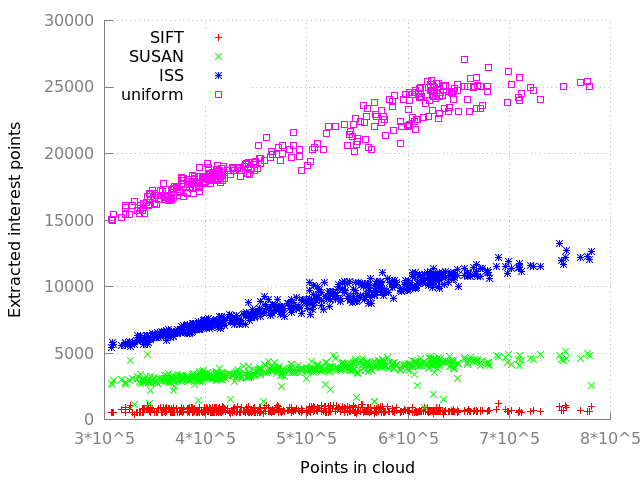
\includegraphics[width=0.8\textwidth]{images/interest_points_0,01}
  \end{center}
\end{frame}
\begin{frame}{Interest points computation time vs. method}
  \begin{center}
    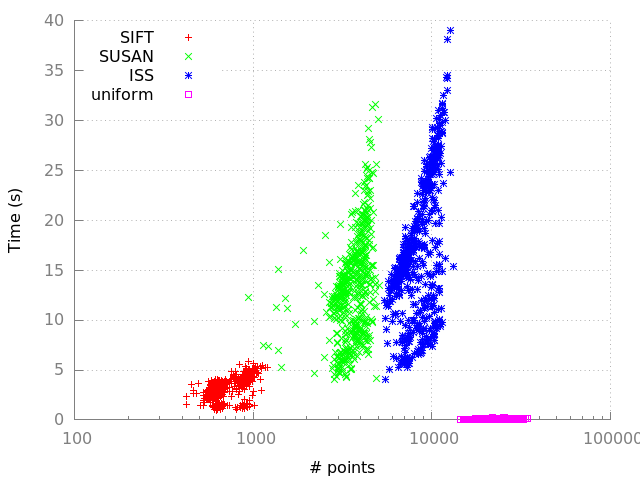
\includegraphics[width=0.8\textwidth]{images/interest_agg_0,01}
  \end{center}
\end{frame}
\begin{frame}{Descriptors computation time (SHOT)}
  \begin{center}
    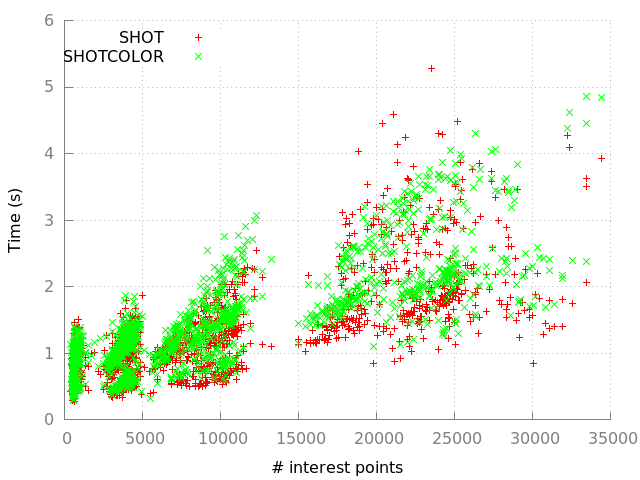
\includegraphics[width=0.8\textwidth]{images/feature_agg_shot_0,01}
  \end{center}
\end{frame}
\begin{frame}{Descriptors computation time (PFH)}
  \begin{center}
    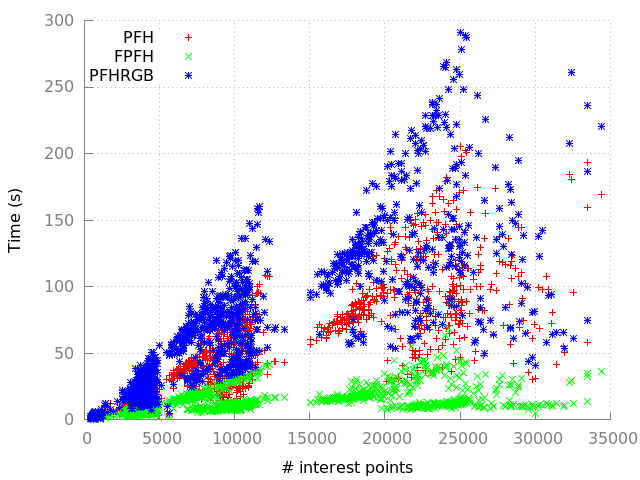
\includegraphics[width=0.8\textwidth]{images/feature_agg_pfh_0,01}
  \end{center}
\end{frame}
\begin{frame}{Query Objects}
  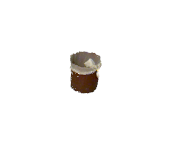
\includegraphics[width=0.15\textwidth]{images/query_trash_bin_front}
  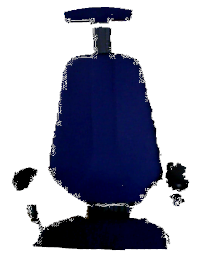
\includegraphics[width=0.15\textwidth]{images/query_chair1_front}
  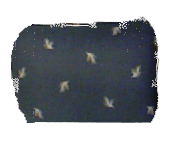
\includegraphics[width=0.15\textwidth]{images/query_pillow_front}
  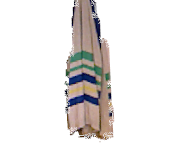
\includegraphics[width=0.15\textwidth]{images/query_hanger_jacket_front}
  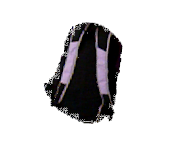
\includegraphics[width=0.15\textwidth]{images/query_backpack2_front}
  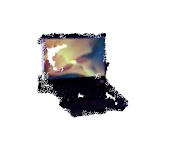
\includegraphics[width=0.15\textwidth]{images/query_laptop1_front}
  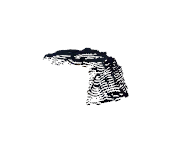
\includegraphics[width=0.15\textwidth]{images/query_top_couch_jacket2_side}
\end{frame}
\begin{frame}{Object Query retrieval rates}
  \begin{table}
    \centering
    \small
    \centerline{
      \begin{tabular}{cc|cc|cc}
        &&\multicolumn{2}{c|}{All} & \multicolumn{2}{c}{\tiny SHOTC,PFHRGB,Uniform,ISS} \\
        Query                             & Setting   & Backpack      & Chair         &Backpack      & Chair         \\\hline
      \multirow{2}{*}{DEF}              & DEF   & 14.2$\pm$22.7 & 29.2$\pm$24.4 &31.1$\pm$28.6 & 39.9$\pm$31.2 \\
                                        & DT    & 18.0$\pm$25.6 & 33.0$\pm$24.4 &40.5$\pm$28.3 & 50.8$\pm$29.2 \\\hline
      \multirow{2}{*}{K10R2}            & DEF   & 18.1$\pm$22.2 & 40.4$\pm$33.1 &30.5$\pm$28.0 & 43.4$\pm$34.8 \\
                                        & DT    & \textbf{21.7}$\pm$24.6 & 49.9$\pm$29.1 &\textbf{39.7}$\pm$28.5 & 56.3$\pm$31.5 \\\hline
      \multirow{2}{*}{K10R25}           & DEF   & 12.2$\pm$16.6 & 40.2$\pm$33.4 &20.6$\pm$22.1 & 44.5$\pm$34.9 \\
                                        & DT    & 19.3$\pm$22.3 & \textbf{53.3}$\pm$30.1 &35.8$\pm$26.1 & \textbf{57.2}$\pm$31.4 \\
      \multicolumn{2}{r|}{Actual counts} & 79    &  85           & 79            & 85
    \end{tabular}
    }
  \end{table}
\end{frame}
\begin{frame}{Object query retrieval rates (DT/DEF), descriptor}
  \begin{table}
    \small
    \centering
    \centerline{
    \begin{tabular}{cc|cccc}
      Object & Descriptor & Top & Total & Unique & Actual \\\hline
      \multirow{5}{*}{Backpack} & FPFH & 2.7$\pm$1.5 & 3.3$\pm$2.5 & 3.3$\pm$2.5 & 80\\
             & PFH & 1.0$\pm$1.0 & 2.3$\pm$3.2 & 2.3$\pm$3.2 & \ditto\\
             & PFHRGB & \textbf{49.3}$\pm$7.2 & \textbf{56.0}$\pm$13.2 & \textbf{56.0}$\pm$13.2 & \ditto\\
             & SHOT & 2.7$\pm$3.8 & 3.3$\pm$4.9 & 3.3$\pm$4.9 & \ditto\\
             & SHOTCOLOR & 9.3$\pm$8.6 & 25.0$\pm$33.3 & 25.0$\pm$33.3 & \ditto\\\hline
      \multirow{5}{*}{Chair} & FPFH & 15.0$\pm$6.2 & 21.7$\pm$10.1 & 21.7$\pm$10.1 & 85\\
             & PFH & 10.0$\pm$9.3 & 17.8$\pm$12.3 & 17.2$\pm$11.6 & \ditto\\
             & PFHRGB & \textbf{36.7}$\pm$18.9 & \textbf{60.7}$\pm$39.6 & \textbf{54.0}$\pm$33.8 & \ditto\\
             & SHOT & 8.3$\pm$9.1 & 29.7$\pm$19.7 & 29.7$\pm$19.7 & \ditto\\
             & SHOTCOLOR & 25.7$\pm$21.1 & 55.0$\pm$37.3 & 47.7$\pm$30.9 & \ditto\\\hline
    \end{tabular}
    }
  \end{table}
\end{frame}
\begin{frame}{Object query retrieval rates (DT/K10R2), descriptor}
  \begin{table}
    \small
    \centerline{
      \begin{tabular}{cc|cccc}
        Object & Descriptor & Top & Total & Unique & Actual \\\hline
        \multirow{5}{*}{Backpack} & FPFH & 2.7$\pm$1.5 & 13.0$\pm$14.8 & 13.0$\pm$14.8 & 80 \\
               & PFH & 2.0$\pm$2.6 & 12.3$\pm$16.4 & 12.3$\pm$16.4 & \ditto\\
               & PFHRGB & \textbf{42.3}$\pm$11.0 & \textbf{53.3}$\pm$19.7 & \textbf{53.3}$\pm$19.7 & \ditto\\
               & SHOT & 1.0$\pm$1.7 & 4.0$\pm$6.9 & 4.0$\pm$6.9 & \ditto\\
               & SHOTCOLOR & 6.7$\pm$5.5 & 26.0$\pm$32.9 & 26.0$\pm$32.9 & \ditto\\\hline
        \multirow{5}{*}{Chair} & FPFH & 16.0$\pm$7.8 & 43.7$\pm$28.4 & 42.0$\pm$27.1 & 85\\
               & PFH & 10.7$\pm$10.0 & 45.0$\pm$30.3 & 43.0$\pm$28.6 & \ditto\\
               & PFHRGB & \textbf{38.0}$\pm$15.7 & \textbf{70.0}$\pm$41.6 & \textbf{59.0}$\pm$32.0 & \ditto\\
               & SHOT & 6.3$\pm$6.5 & 55.7$\pm$43.7 & 51.7$\pm$39.8 & \ditto \\
               & SHOTCOLOR & 25.3$\pm$21.7 & 62.3$\pm$45.5 & 53.7$\pm$37.9 & \ditto\\\hline
      \end{tabular}
    }
  \end{table}
\end{frame}
\begin{frame}{Object query retrieval rates (DT/DEF), interest}
  \begin{table}
    \centerline{
      \begin{tabular}{cc|ccccc}
        Object & Interest & Top & Total & Unique & Actual \\\hline
        \multirow{4}{*}{Backpack} & ISS & \textbf{16.8}$\pm$21.6 & \textbf{30.0}$\pm$31.5 & \textbf{30.0}$\pm$31.5 & 80\\
               & SIFT & 1 & 1 & 1 & \ditto\\
               & SUSAN & 10.8$\pm$17.5 & 10.8$\pm$17.5 & 10.8$\pm$17.5 & \ditto\\
               & UNIFORM & 14.0$\pm$26.0 & 16.2$\pm$29.9 & 16.2$\pm$29.9 & \ditto\\\hline
        \multirow{4}{*}{Chair} & ISS & 15.0$\pm$18.0 & 50.0$\pm$27.6 & 46.2$\pm$22.6 &85\\
               & SIFT & 5 & 5 & 5 & \ditto\\
               & SUSAN & 10.8$\pm$2.9 & 10.8$\pm$2.9 & 10.8$\pm$2.9 & \ditto\\
               & UNIFORM & \textbf{32.6}$\pm$16.0 & \textbf{52.6}$\pm$26.1 & \textbf{47.6}$\pm$20.6 & \ditto\\\hline
      \end{tabular}
    }
  \end{table}
\end{frame}
\begin{frame}{Object query retrieval rates (DT/K10R2), interest}
  \begin{table}
    \centerline{
      \begin{tabular}{cc|cccc}
        Object & Interest & Top & Total & Unique & Actual \\\hline
        \multirow{3}{*}{Backpack} & ISS & \textbf{15.4}$\pm$21.3 & \textbf{41.0}$\pm$24.1 & \textbf{41.0}$\pm$24.1 & 80\\
               & SUSAN & 8.2$\pm$13.1 & 8.2$\pm$13.1 & 8.2$\pm$13.1 & \ditto\\
               & UNIFORM & 9.2$\pm$18.9 & 16.0$\pm$25.3 & 16.0$\pm$25.3 & \ditto\\\hline
        \multirow{3}{*}{Chair} & ISS & 14.2$\pm$16.6 & 77.2$\pm$15.5 & 69.4$\pm$8.3 & 85\\
               & SUSAN & 11.4$\pm$5.7 & 11.8$\pm$6.0 & 11.8$\pm$6.0 & \ditto\\
               & UNIFORM & \textbf{32.2}$\pm$17.7 & \textbf{77.0}$\pm$16.3 & \textbf{68.4}$\pm$11.6& \ditto\\\hline
      \end{tabular}
    }
  \end{table}
\end{frame}
\begin{frame}
  \begin{figure}
    \centering
    \centerline{
      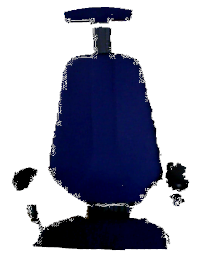
\includegraphics[width=0.18\textwidth]{images/query_chair1_front}
      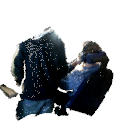
\includegraphics[width=0.18\textwidth]{images/queryresults/chair_0}
      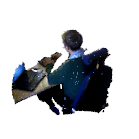
\includegraphics[width=0.18\textwidth]{images/queryresults/chair_1}
      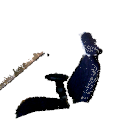
\includegraphics[width=0.18\textwidth]{images/queryresults/chair_2}
      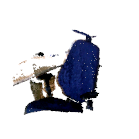
\includegraphics[width=0.18\textwidth]{images/queryresults/chair_3}
      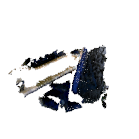
\includegraphics[width=0.18\textwidth]{images/queryresults/chair_4}
    }\\
    \centerline{
      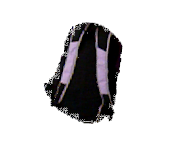
\includegraphics[width=0.18\textwidth]{images/query_backpack2_front}
      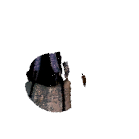
\includegraphics[width=0.18\textwidth]{images/queryresults/backpack_0}
      \includegraphics[width=0.18\textwidth]{images/queryresults/backpack_1}
      \includegraphics[width=0.18\textwidth]{images/queryresults/backpack_2}
      \includegraphics[width=0.18\textwidth]{images/queryresults/backpack_3}
      \includegraphics[width=0.18\textwidth]{images/queryresults/backpack_4}
    }\\
    \centerline{
      \includegraphics[width=0.18\textwidth]{images/query_hanger_jacket_front}
      \includegraphics[width=0.18\textwidth]{images/queryresults/hanger_jacket_0}
      \includegraphics[width=0.18\textwidth]{images/queryresults/hanger_jacket_1}
      \includegraphics[width=0.18\textwidth]{images/queryresults/hanger_jacket_2}
      \includegraphics[width=0.18\textwidth]{images/queryresults/hanger_jacket_3}
      \includegraphics[width=0.18\textwidth]{images/queryresults/hanger_jacket_4}
    }\\
    \centerline{
      \includegraphics[width=0.18\textwidth]{images/query_laptop1_front}
      \includegraphics[width=0.18\textwidth]{images/queryresults/laptop_0}
      \includegraphics[width=0.18\textwidth]{images/queryresults/laptop_1}
      \includegraphics[width=0.18\textwidth]{images/queryresults/laptop_2}
      \includegraphics[width=0.18\textwidth]{images/queryresults/laptop_3}
      \includegraphics[width=0.18\textwidth]{images/queryresults/laptop_4}
    }
  \end{figure}
\end{frame}
\section{Conclusion}
\begin{frame}{Conclusion}
  Successfully implemented a system for object retrieval
  \begin{itemize}
  \item Best results (50\% retrieved objects) were with uniform interest point
    selection and PFHRGB descriptor.
  \item Some of the objects were not retrievable or had very low retrieval rates
    (10\%). Perhaps due to size, shape or preprocessing issues?
  \item Might be possible to perform better with tweaks, but wouldn't work as a standalone system
  \end{itemize}
\end{frame}
\begin{frame}
  \begin{center}
    \huge Questions?
  \end{center}
\end{frame}
\end{document}
